\documentclass{ieeeaccess}
\usepackage{cite}
\usepackage{amsmath,amssymb,amsfonts}
\usepackage{graphicx}
\usepackage{textcomp}
\usepackage{bm}
\usepackage{booktabs}
\usepackage{multirow}
\usepackage{url}

\makeatletter
\AtBeginDocument{\DeclareMathVersion{bold}
\SetSymbolFont{operators}{bold}{T1}{times}{b}{n}
\SetSymbolFont{NewLetters}{bold}{T1}{times}{b}{it}
\SetMathAlphabet{\mathrm}{bold}{T1}{times}{b}{n}
\SetMathAlphabet{\mathit}{bold}{T1}{times}{b}{it}
\SetMathAlphabet{\mathbf}{bold}{T1}{times}{b}{n}
\SetMathAlphabet{\mathtt}{bold}{OT1}{pcr}{b}{n}
\SetSymbolFont{symbols}{bold}{OMS}{cmsy}{b}{n}
\renewcommand\boldmath{\@nomath\boldmath\mathversion{bold}}}
\makeatother

\def\BibTeX{{\rm B\kern-.05em{\sc i\kern-.025em b}\kern-.08em
    T\kern-.1667em\lower.7ex\hbox{E}\kern-.125emX}}

\begin{document}
\history{Manuscript revised August 10, 2026.}
\doi{}

\title{PGA-UNet: A Lightweight Prompt-Guided Attention U-Net for Interactive Bone X-Ray Lesion Segmentation}
\author{\uppercase{Thong Luc}\authorrefmark{1},
\uppercase{Huu-Binh Nguyen}\authorrefmark{1},
\uppercase{Ly Quoc Ngoc}\authorrefmark{2}}

\address[1]{B.Sc. Program in Computer Science, Faculty of Information Technology, University of Science, VNU-HCM, Vietnam}
\address[2]{[ Th\`ay \dj i\`en th\^ong tin gi\'up em: affiliation ]}

\markboth
{Luc \headeretal: PGA-UNet for Interactive Bone X-Ray Lesion Segmentation}
{Luc \headeretal: PGA-UNet for Interactive Bone X-Ray Lesion Segmentation}

\corresp{Corresponding author: Thong Luc (e-mail: 22120196@student.hcmus.edu.vn).}

\begin{abstract}
Bone X-ray lesion segmentation remains difficult because lesions are often small, low-contrast, and anatomically confounded, so fully automatic segmentation models may fail before accurate boundary prediction becomes possible. Prior studies addressed this problem either with automatic encoder-decoder networks such as U-Net and Attention U-Net or with promptable foundation models such as SAM-Med2D. However, automatic models do not exploit user-provided spatial guidance, whereas foundation models are computationally heavy and do not necessarily preserve prompt influence throughout a lightweight task-specific network. This article proposes PGA-UNet, a lightweight prompt-guided convolutional architecture that converts a bounding-box prompt into a Gaussian-smoothed plateau heatmap, amplifies prompt-relevant encoder features through a Prompt Spatial Gate (PSG), and conditions decoder skip attention through a Conditional Attention Decoder (CAD). On BTXRD and FracAtlas, PGA-UNet achieved Dice scores of 0.8607 and 0.8169 at $512\times512$, respectively. In a matched $256\times256$ comparison, PGA-UNet outperformed fine-tuned SAM-Med2D under both covering and off-center prompts on both datasets, with the clearest advantage on the 50 smallest BTXRD lesions. Ablation results further showed that the Gaussian prompt, PSG, and CAD each improved robustness, with the full combination providing the strongest overall behavior. PGA-UNet uses 2.95M parameters, corresponding to an approximately 92-fold reduction relative to SAM-Med2D in the tested $256\times256$ setting. These results indicate that prompt information is most effective in this task when it is both spatially softened and propagated throughout the network from early encoding to late decoding.
\end{abstract}

\begin{keywords}
bone X-ray, interactive segmentation, medical image segmentation, prompt-guided learning, Attention U-Net
\end{keywords}

\titlepgskip=-15pt
\maketitle

\section{Introduction}
\label{sec:introduction}
\PARstart{B}{one} X-ray imaging is widely used in screening, diagnosis support, and follow-up because it is fast, inexpensive, and broadly available. However, lesion segmentation in radiographs remains difficult because targets may be small, low-contrast, elongated, or partially occluded by surrounding anatomy. In such cases, the main failure often occurs at localization: if the model attends to the wrong anatomical region, accurate boundary prediction becomes irrelevant.

This difficulty motivated two broad development lines in prior work. One line improved fully automatic segmentation networks, beginning with U-Net-style encoder-decoder architectures and later extending them with attention mechanisms such as Attention U-Net \cite{b3,b4}. These models remain strong and efficient baselines, but they still solve a harder problem than many practical workflows require, namely localizing and segmenting every lesion from scratch. A second line moved toward interactive or prompt-guided segmentation, where clicks, scribbles, geodesic cues, or boxes are provided by the user \cite{b5,b6}. More recently, promptable foundation models such as SAM and SAM-Med2D pushed this direction further \cite{b1,b2}. Although powerful, these models are heavy and may be unnecessarily expensive for a fixed grayscale radiograph task with repeated low-latency interaction.

In the present setting, a clinician can often provide a coarse bounding box more easily than a fully automatic system can localize a small lesion reliably. This creates a more focused research question: how should a lightweight model use that coarse spatial cue? A simple answer is to concatenate the prompt as an extra channel. However, that strategy does not guarantee that the prompt remains influential once features move deeper through the network, especially when the prompt is slightly misaligned or when lesion evidence is weak.

This article therefore investigates a lightweight alternative. We propose PGA-UNet, a prompt-guided convolutional architecture that treats the box prompt as a structured spatial prior rather than as a simple auxiliary channel. The prompt is encoded as a plateau-style Gaussian heatmap, injected into encoder features through a Prompt Spatial Gate (PSG), and reused in the decoder through a Conditional Attention Decoder (CAD). The underlying encoder-decoder structure remains U-Net-like, but prompt information is not limited to the input layer; it is amplified and maintained throughout the network.

The main contributions of this article are as follows.
\begin{itemize}
\item We present a compact prompt-guided architecture for interactive bone X-ray lesion segmentation.
\item We integrate plateau-style Gaussian prompting, encoder-side prompt gating, and decoder-side prompt-conditioned attention within a lightweight network.
\item We formulate an offline training and online interactive inference framework for prompt-guided radiographic lesion segmentation, with explicit mathematical definitions for prompt encoding, encoder gating, and decoder conditioning.
\item We evaluate the method on BTXRD and FracAtlas under covering and off-center prompt settings, including comparisons with Attention U-Net and SAM-Med2D, a small-lesion analysis, Monte Carlo cross-validation, and efficiency measurements.
\item We report ablation, efficiency, and small-lesion results that clarify where the proposed prompt-conditioning design is most useful.
\end{itemize}

\section{Related Work}
Automatic medical image segmentation progressed from fully convolutional encoder-decoder architectures toward more selective skip-feature processing. U-Net established the canonical multi-scale encoder-decoder template for biomedical segmentation \cite{b3}. Attention U-Net then introduced attention gates on skip connections so that decoder-side fusion could suppress irrelevant spatial responses more selectively \cite{b4}. This line of work improved automatic segmentation quality, but it still assumes that the network itself must both localize and segment the lesion from the raw image alone.

Interactive medical segmentation developed in parallel from the observation that partial user guidance can simplify the problem substantially \cite{b5,b6}. Early methods used clicks, scribbles, and geodesic cues; later work incorporated boxes as practical coarse prompts. The next major step was promptable foundation models such as SAM, SAM-Med2D, and MedSAM, which generalized prompt-driven segmentation across many medical domains \cite{b1,b2,b9}. These models are flexible, but their prompt usage is architecturally different from lightweight task-specific CNNs, and their computational cost is much higher. For very small radiographic lesions, another unresolved issue is whether a coarse prompt merely indicates the approximate region or whether it continues to shape feature extraction and decoding throughout the network.

The present work is motivated by that gap. In grayscale bone radiographs, the challenge is not only to know \emph{where} the lesion roughly is, but also to preserve weak lesion evidence while suppressing surrounding clutter. A lightweight prompt-guided CNN may therefore benefit from making prompt information active from early encoding to late decoding instead of using the prompt only as an initial cue.

\begin{table}[t]
\caption{Representative prior work and the remaining gap addressed in this article.}
\label{tab:related}
\centering
\scriptsize
\resizebox{\columnwidth}{!}{%
\begin{tabular}{p{1.9cm}p{2.2cm}p{2.7cm}p{2.7cm}p{2.1cm}p{2.1cm}}
\toprule
Work & Principle & Method & Performance Evidence & Pros & Cons \\
\midrule
U-Net \cite{b3} & Fully convolutional encoder-decoder & Multi-scale skip-connected segmentation network & Broad biomedical benchmarks; Dice-based overlap reporting & Simple, efficient, strong canonical baseline & No prompt guidance; all localization must be automatic \\
\midrule
Attention U-Net \cite{b4} & Skip-feature filtering by attention gates & U-Net with gated skip connections & Medical image segmentation tasks with overlap metrics such as Dice and IoU & Stronger automatic baseline than plain U-Net & Attention is still learned without explicit prompt conditioning \\
\midrule
DeepIGeoS and related interactive methods \cite{b6} & User guidance reduces search space & Geodesic or interaction-aware segmentation & Interactive medical segmentation under user input & Better reflects clinical interaction & Interaction mechanism can be task-specific or expensive to maintain \\
\midrule
SAM-Med2D / MedSAM \cite{b2,b9} & Promptable foundation segmentation & Large pretrained model with prompt-driven mask decoding & Multi-dataset medical evaluation with prompt-based metrics & Flexible and broadly applicable & Heavy; prompt influence is not designed as a lightweight end-to-end radiograph-specific prior \\
\midrule
This work & Prompt as a dense spatial prior throughout the network & Gaussian plateau prompt + PSG + CAD in a lightweight CNN & BTXRD and FracAtlas; Dice, IoU, HD95, CBL, efficiency, small-lesion analysis & Lightweight, prompt-aware from encoder to decoder, robust to prompt perturbation & Still requires supervised masks and fixed-resolution preprocessing \\
\bottomrule
\end{tabular}
}
\end{table}

\section{Method}
\subsection{Offline and Online Framework}
The proposed system has two stages. In the offline stage, the model is trained on radiographs paired with lesion polygons. Each polygon is converted into a training prompt by generating a simulated bounding box and then transforming that box into a Gaussian-smoothed plateau heatmap. The network learns to map the image-prompt pair to the binary lesion mask. In the online stage, a user provides a coarse bounding box around a suspected lesion on a new radiograph. The same prompt-construction procedure is applied, and the trained model predicts the final lesion mask.

The scientific contribution of this framework is that the prompt is not treated as an optional side input used only at the first layer. Instead, the prompt is encoded as a dense spatial prior and made active at both encoder and decoder stages. The practical consequence is improved robustness when the prompt is coarse, mildly off-center, or applied to a very small lesion.

\subsection{Problem Setting}
Given a grayscale radiograph $\mathbf{I}\in\mathbb{R}^{H\times W}$ and a user-provided bounding box $\mathbf{B}$, the goal is to predict a binary lesion mask $\hat{\mathbf{M}}$. Let $\mathbf{H}(\mathbf{B})$ be the prompt heatmap derived from the box. PGA-UNet predicts
\begin{equation}
\hat{\mathbf{M}} = \mathbf{1}\left[f_{\mathrm{PGA}}\left(\mathbf{I},\mathbf{H}(\mathbf{B});\theta\right)\ge 0.5\right].
\end{equation}

\subsection{Prompt Representation}
The input prompt is not encoded as a hard binary rectangle. Instead, the box interior is converted into a plateau map and its boundaries are softened with Gaussian filtering. In the implementation used for the reported experiments, the box is first assigned a minimum prompt margin before rasterization and then smoothed with a Gaussian kernel. At $256\times256$, the minimum margin is 5 pixels and the kernel size is $31\times31$; at $512\times512$, the corresponding values are 10 pixels and $61\times61$. This preserves the full spatial extent of the region of interest while reducing over-dependence on an abrupt boundary.

During evaluation, prompts are tested in two settings. A covering prompt expands the lesion bounding box by 15\%--45\% of lesion width and height. An off-center prompt first applies the same expansion and then shifts the box by up to 30\% of lesion width and height while still covering the lesion. A single model is trained per dataset and resolution; the prompt condition is varied only at evaluation time unless otherwise stated in the ablation study.

Let $(x_1,y_1,x_2,y_2)$ denote the tight lesion box and let $w=x_2-x_1$ and $h=y_2-y_1$. The simulated covering box expands each side by a random fraction in $[0.15,0.45]$ of $w$ or $h$ during training and by a fixed fraction of 0.30 during evaluation. The off-center box applies the same expansion and then adds a translation bounded by $0.30w$ horizontally and $0.30h$ vertically while preserving lesion coverage. This simulation is not a substitute for radiologist-drawn prompts, but it provides a controlled way to test sensitivity to plausible box variation.

Algorithmically, prompt construction follows four steps: 1) derive a lesion box from the polygon annotation or user input, 2) enlarge that box with a resolution-aware minimum margin, 3) rasterize the enlarged region into a plateau mask, and 4) smooth the plateau boundary with a Gaussian kernel. This sequence avoids the hard-edge dependence of a binary box while preserving a clear spatial prior.

\subsection{Prompt Spatial Gate}
Let $\mathbf{x}^{l}$ denote the encoder feature map at level $l$. PSG modulates it with a prompt-derived attention map $\mathbf{A}^{l}_{\mathrm{PSG}}$:
\begin{equation}
\widetilde{\mathbf{x}}^{l}
=
\mathbf{x}^{l}\odot
\left(1+\alpha^{l}_{\mathrm{PSG}}\mathbf{A}^{l}_{\mathrm{PSG}}\right),
\end{equation}
where $\odot$ is element-wise multiplication and $\alpha^{l}_{\mathrm{PSG}}$ is learnable. In the implementation, $\alpha^{l}_{\mathrm{PSG}}$ is initialized to 0.1 and clamped to $[0,1]$. The residual form keeps the original feature stream available while emphasizing prompt-relevant regions.

\subsection{Conditional Attention Decoder}
CAD extends decoder attention by conditioning the skip gate on prompt-encoded features. Let $\mathbf{g}^{l}$ be the decoder gating feature and $\mathbf{p}^{l}_{\mathrm{enc}}$ the prompt encoding at the same scale. The conditioned gate is
\begin{equation}
\mathbf{g}'^{\,l}=\mathbf{g}^{l}+c^{l}\alpha^{l}_{\mathrm{CAD}}w_{l}\mathbf{p}^{l}_{\mathrm{enc}},
\end{equation}
where $c^{l}$ is a prompt confidence scalar, $\alpha^{l}_{\mathrm{CAD}}$ is learnable, and $w_{l}$ is a fixed depth coefficient. This design helps the decoder remain aligned with the prompt even when the box is not perfectly centered.

The prompt encoder in CAD uses two $3\times3$ convolutions with instance normalization and ReLU. The prompt-confidence scalar $c^{l}$ is produced by global average pooling followed by a $1\times1$ convolution and a sigmoid nonlinearity. The decoder depth coefficients are fixed to $\{1.0,0.7,0.4,0.2\}$ from deep to shallow layers. With feature scale 4, the channel widths are $\{16,32,64,128,256\}$ from the shallowest encoder stage to the bottleneck. The CAD mixing coefficient is parameterized as a sigmoid-transformed scalar and initialized near 0.3.

Taken together, the method can be summarized as follows: 1) preprocess the image and prompt into a common square resolution, 2) encode prompt-relevant spatial priors with PSG in the encoder, 3) propagate prompt-conditioned context through CAD in the decoder, and 4) predict the final binary lesion mask. The scientific meaning of the contribution is that prompt information is both spatially softened and repeatedly reused, rather than being injected once and left to dissipate.

\begin{figure}[t]
\centering
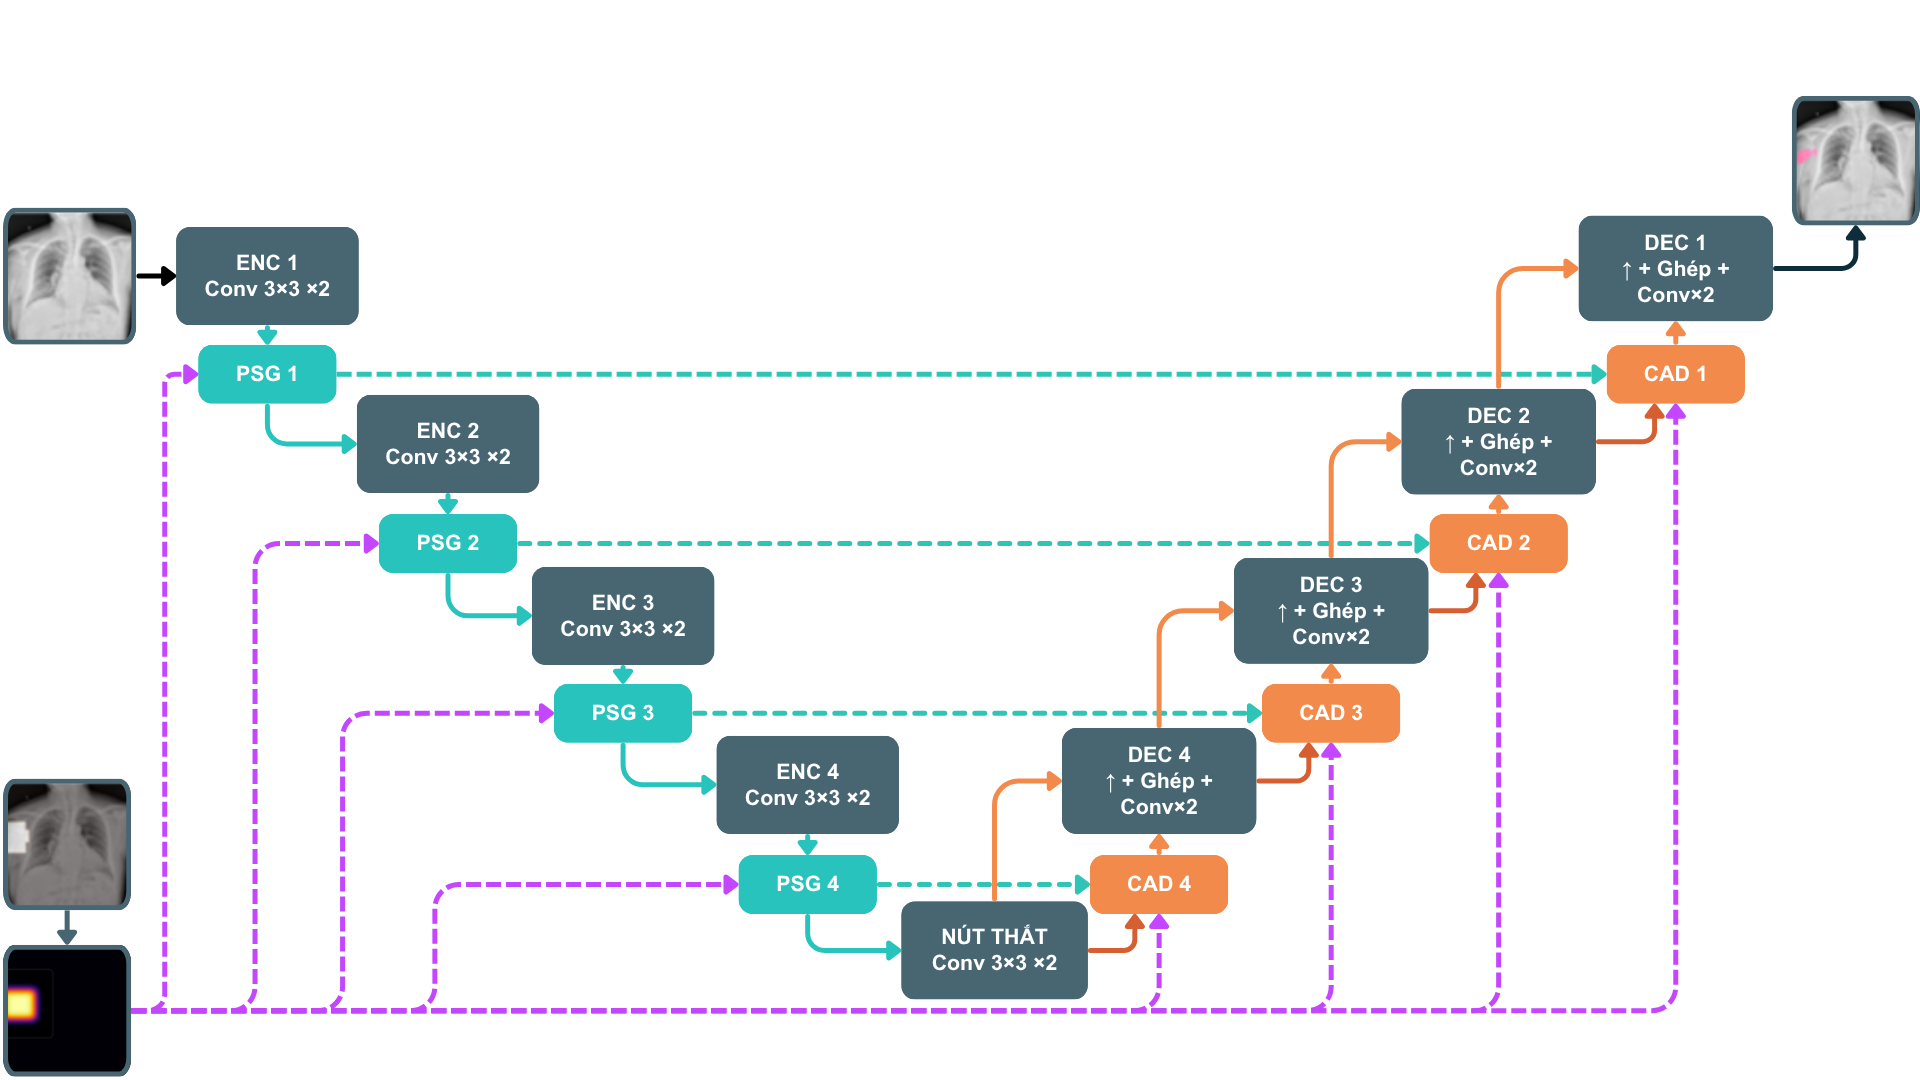
\includegraphics[width=\columnwidth]{images/architecture_pga_unet.png}
\caption{Overview of PGA-UNet. Prompt information derived from the bounding box is injected into encoder features through PSG and reused in decoder skip attention through CAD.}
\label{fig:arch}
\end{figure}

\section{Experimental Setup}
\subsection{Datasets}
We evaluate on two public bone radiograph datasets. BTXRD is a primary bone tumor X-ray dataset with polygon annotations for classification, localization, and segmentation \cite{b7}. Our BTXRD split contains 1,493/187/187 images with 1,848/238/232 lesion polygons for training, validation, and testing, respectively. FracAtlas is a fracture radiograph dataset with classification, localization, and segmentation labels \cite{b8}. After data cleaning and polygon normalization, our FracAtlas split contains 573/72/72 images with 730/95/92 lesion polygons for training, validation, and testing, respectively.

Splits are performed at the image level, and all polygons from the same image are kept in the same split. The public metadata were insufficient to verify strict patient-level separation. Each polygon is treated as one promptable lesion sample during training. For image-level evaluation, if an image contains multiple lesions, the model is run once per lesion box and the probability maps are merged by pixelwise maximum before thresholding at 0.5. Ground-truth masks are merged by union in the same image.

Inputs are resized isotropically and padded to square resolutions of $256\times256$ or $512\times512$ to preserve aspect ratio. Images, masks, and prompt maps undergo the same geometric preprocessing.

\subsection{Training Details}
All CNN models were implemented in PyTorch and trained on an NVIDIA Tesla T4 GPU with 16 GB memory. PGA-UNet and Attention U-Net were trained separately on each dataset and resolution. The optimizer was AdamW with learning rate $10^{-4}$ and weight decay $10^{-4}$. The loss was the sum of binary cross-entropy and Dice loss. Batch size was 4, the maximum training budget was 100 epochs, and early stopping with patience 15 was used. The primary model-selection criterion was validation Dice under the covering-prompt condition.

Training-time augmentation included horizontal flipping and random rotation within $\pm15^\circ$. The implementation also applied prompt dropout or prompt noise to a subset of training iterations to reduce over-reliance on an ideal prompt. For the fine-tuned SAM-Med2D comparison, the pretrained image encoder was frozen except for its lightweight Adapter layers, while the prompt encoder and mask decoder were fully updated on each dataset under the same split protocol. Rather than the original authors' training-time box perturbation, a tight box with a few pixels of random jitter combined with iterative point-based refinement, SAM-Med2D was finetuned box-only, with each training box drawn from the same covering-prompt protocol used for PGA-UNet: an independent random expansion of 15\%--45\% per side on half of the samples, or the same expansion followed by an off-center shift of up to 30\% on the other half. Matching the training-time prompt distribution between the two models avoids confounding architectural differences with a train-test distribution shift, since evaluating SAM-Med2D under PGA-UNet's wider covering prompts while training it only on the authors' narrow box jitter would otherwise penalize it for a distribution mismatch unrelated to architecture. Validation during SAM-Med2D finetuning and the final test split used the same covering-prompt protocol as PGA-UNet, with batch size 4, a maximum of 100 epochs, early stopping with patience 30, and learning rate $10^{-5}$. Additional stability experiments were performed using Monte Carlo cross-validation, that is, repeated random image-level splits rather than strict non-overlapping $k$-fold partitioning.

Two evaluation details are important for interpreting the results. First, prompt generation is resolution-aware: at $256\times256$ the minimum prompt margin is 5 pixels with a Gaussian kernel size of 31, while at $512\times512$ the corresponding values are 10 pixels and 61. Second, the Monte Carlo cross-validation experiments are auxiliary stability evidence rather than replacements for the fixed train/validation/test split used in the main tables.

\subsection{Baselines and Metrics}
PGA-UNet is compared with Attention U-Net \cite{b4} as the main automatic baseline and with SAM-Med2D \cite{b2} as the main prompt-based baseline. Attention U-Net is trained without prompts, whereas SAM-Med2D is evaluated at $256\times256$ in fine-tuned form with the same dataset splits and the same box prompts as PGA-UNet.

We report Dice, IoU, precision, recall, HD95, and center-based localization (CBL). For a predicted mask centroid $(x_p,y_p)$, a ground-truth centroid $(x_g,y_g)$, and the diagonal length $D_{\mathrm{GT}}$ of the ground-truth bounding box, CBL is defined as
\begin{equation}
\mathrm{CBL}=\max\left(0,1-\frac{\sqrt{(x_p-x_g)^2+(y_p-y_g)^2}}{D_{\mathrm{GT}}}\right).
\end{equation}
HD95 is computed from bidirectional boundary distances. If both masks are empty, HD95 is set to 0. If exactly one mask is empty, HD95 is set to the image side length (256 or 512 pixels). No samples are discarded.

\subsection{Scope of Analysis}
This article focuses on prompt-guided segmentation itself and excludes the auxiliary screening pipeline explored separately in the thesis manuscript. To keep the article compact, we retain only the subgroup analyses that most directly support the main claim: robustness under imperfect prompts and effectiveness on small lesions.

\section{Results}
\subsection{Main Comparison Across Datasets and Resolutions}
This first group of experiments addresses the most basic question: does PGA-UNet remain effective across both datasets, across both tested input resolutions, and across both prompt scenarios? These experiments primarily validate the main system-level contribution, namely that prompt-conditioned processing through both encoder and decoder can be transferred across two radiographic datasets with different lesion characteristics. PGA-UNet performs well on both BTXRD and FracAtlas under the intended workflow with coarse box guidance. Across the main experiments, the model remains competitive at both $256\times256$ and $512\times512$ and under both covering and off-center prompt settings. The consistent trend across datasets, resolutions, and prompt scenarios is that explicit prompt conditioning in both the encoder and decoder remains useful even when lesion appearance changes substantially between the two datasets.


\subsection{Effect of Input Resolution}
This experiment isolates the contribution of image resolution within the same architecture and prompt protocol. It supports the claim that the proposed method is especially useful when small lesion evidence would otherwise be weakened by downsampling. The thesis experiments therefore trained PGA-UNet independently at $256\times256$ and $512\times512$ on each dataset. The higher resolution consistently improved Dice, but the gain was larger on BTXRD than on FracAtlas. This difference is consistent with the datasets themselves: BTXRD contains many small or irregular lesions whose local evidence degrades noticeably after aggressive downsampling, whereas FracAtlas more often contains elongated but visually simpler fracture structures.

\begin{table}
\caption{PGA-UNet Dice under covering and off-center prompts at two resolutions.}
\label{tab:resolution}
\centering
\resizebox{\columnwidth}{!}{%
\begin{tabular}{llcc}
\toprule
Dataset & Resolution & Covering & Off-center \\
\midrule
BTXRD & $256\times256$ & 0.8433 & 0.8150 \\
BTXRD & $512\times512$ & \textbf{0.8607} & \textbf{0.8423} \\
\midrule
FracAtlas & $256\times256$ & 0.8110 & 0.7842 \\
FracAtlas & $512\times512$ & \textbf{0.8169} & \textbf{0.7850} \\
\bottomrule
\end{tabular}
}
\end{table}

The resolution comparison should not be overinterpreted as a pure image-size effect because the prompt representation also changes with resolution through its margin and Gaussian smoothing scale. Even with that caveat, the main trend remains useful: prompt-guided segmentation of small radiographic lesions benefits from preserving more spatial detail, especially when the lesion occupies only a tiny fraction of the image.


\subsection{Monte Carlo Cross-Validation}
This experiment examines whether the main findings remain stable when the image-level split is redrawn repeatedly under limited data. It supports the robustness claim at the dataset-partition level rather than at the prompt-perturbation level. Supplementary experiments therefore used Monte Carlo cross-validation, that is, repeated random image-level splits. These results are not intended to replace the fixed-split main tables, but they provide additional evidence that the $512\times512$ PGA-UNet configuration remains competitive across repeated random repartitions. In the final rerun, this subsection should report mean $\pm$ standard deviation for Dice and the main auxiliary metrics.

\begin{figure}[t]
\centering
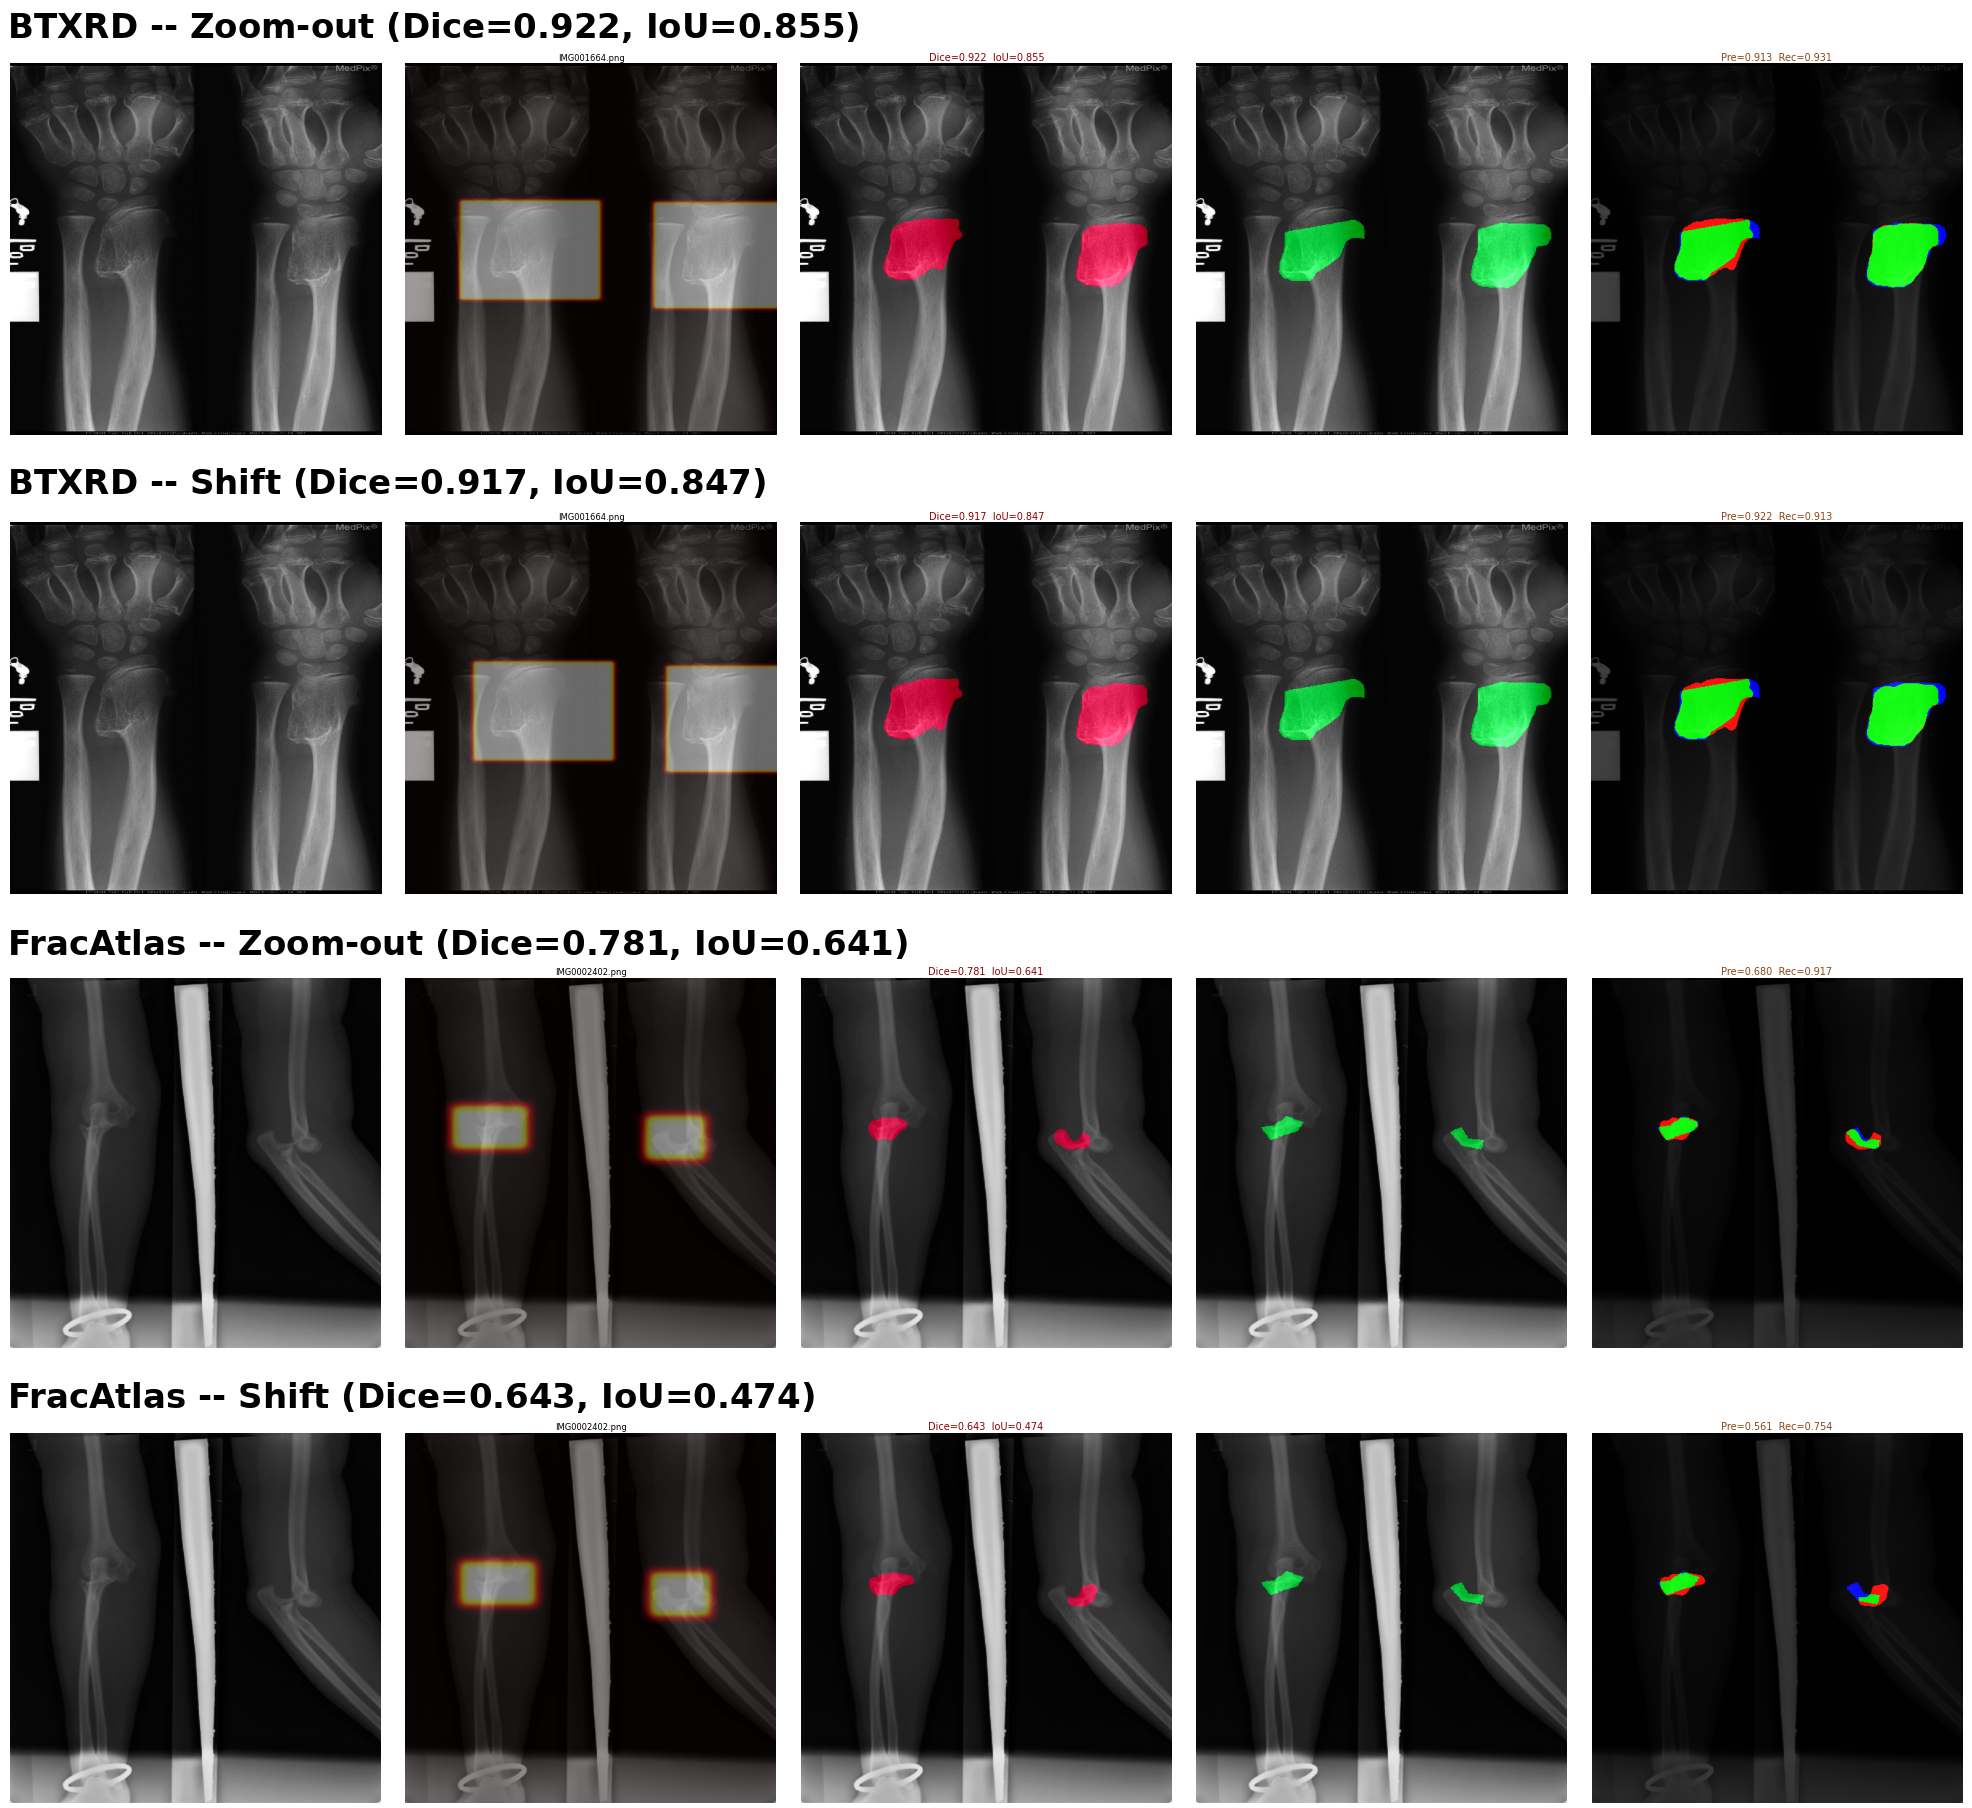
\includegraphics[width=\columnwidth]{images/prompt_robustness_examples.png}
\caption{Qualitative behavior under prompt perturbation. PGA-UNet remains more stable when the prompt is shifted away from the ideal covering box, although thin fracture patterns are still harder than larger compact lesions.}
\label{fig:robust}
\end{figure}


\subsection{Comparison with the Automatic Baseline}
This comparison tests whether the proposed prompt-guided architecture yields a measurable advantage over a strong automatic encoder-decoder baseline. The contribution being examined here is not merely model size, but the use of coarse prompt information throughout the network. Table~\ref{tab:baseline} compares PGA-UNet with Attention U-Net at $512\times512$. This comparison is intentionally between a prompt-guided model and a strong automatic baseline without prompt guidance. PGA-UNet achieves higher system-level segmentation performance when coarse box guidance is available on both BTXRD and FracAtlas.

\begin{table}
\caption{Comparison with the automatic baseline at $512\times512$.}
\label{tab:baseline}
\centering
\resizebox{\columnwidth}{!}{%
\begin{tabular}{llccc}
\toprule
Dataset & Model & Dice & IoU & HD95 \\
\midrule
\multirow{2}{*}{BTXRD}
& Attention U-Net & 0.4122 & 0.3291 & 136.75 \\
& PGA-UNet & \textbf{0.8607} & \textbf{0.7630} & \textbf{12.12} \\
\midrule
\multirow{2}{*}{FracAtlas}
& Attention U-Net & 0.2467 & 0.1816 & 186.46 \\
& PGA-UNet & \textbf{0.8169} & \textbf{0.6953} & \textbf{7.45} \\
\bottomrule
\end{tabular}
}
\end{table}


\subsection{Attention U-Net Top- and Bottom-Dice Subsets}
This subgroup analysis is an extension of the automatic-baseline comparison. After comparing PGA-UNet with Attention U-Net at the dataset level, we ask a more specific question: how does PGA-UNet behave on images where the automatic baseline is relatively strong versus relatively weak? The purpose is to clarify the practical meaning of the Attention U-Net comparison rather than to define objective data difficulty. We therefore compare Attention U-Net top-Dice and bottom-Dice image groups on BTXRD. Specifically, we select the 50 test images with the highest Attention U-Net Dice scores and the 50 test images with the lowest Attention U-Net Dice scores, then re-evaluate PGA-UNet on the same two groups. This analysis does not define intrinsic data difficulty; it only reports performance on subsets induced by the Attention U-Net ranking.

\begin{table}
\caption{Top-Dice and bottom-Dice comparison on BTXRD (50 images per group).}
\label{tab:extreme}
\centering
\resizebox{\columnwidth}{!}{%
\begin{tabular}{llcc}
\toprule
Group & Model & Dice & HD95 \\
\midrule
\multirow{2}{*}{Top-Dice}
& Attention U-Net & 0.8488 & 51.34 \\
& PGA-UNet & \textbf{0.8972} & \textbf{13.20} \\
\midrule
\multirow{2}{*}{Bottom-Dice}
& Attention U-Net & 0.0211 & 284.72 \\
& PGA-UNet & \textbf{0.8261} & \textbf{7.75} \\
\bottomrule
\end{tabular}
}
\end{table}

In the top-Dice group, PGA-UNet still improves over Attention U-Net, increasing Dice from 0.8488 to 0.8972. The larger contrast appears in the bottom-Dice group, where Attention U-Net falls to 0.0211 Dice while PGA-UNet reaches 0.8261. Because the two groups are defined directly from Attention U-Net scores, these values should not be interpreted as global averages; instead, they highlight how PGA-UNet behaves on cases where the automatic baseline is relatively strong or weak.

The qualitative examples help clarify this behavior. In the Attention U-Net top-Dice group, the automatic baseline can often place the predicted mask in roughly the correct anatomical region, but it may still produce spurious responses far from the lesion. Even when the lesion itself is covered reasonably well, those distant false positives reduce overlap-based metrics such as Dice and IoU. PGA-UNet is less prone to this pattern because the bounding box prompt constrains the model to a more relevant spatial region. In the bottom-Dice group, the failure is more severe: the automatic baseline may localize the wrong region or miss the lesion almost entirely. A likely reason is that the attention gate itself has no guarantee of learning a clinically correct gating policy: it filters whatever features it has learned to emphasize, whether those features correspond to lesions or to spurious high-energy structures. When the learned response is dominated by background clutter or artifact-like signals with strength comparable to, or larger than, the true lesion evidence, the gate can no longer rescue localization. In practice, it may suppress only mild background activity while remaining ineffective against stronger false responses. In contrast, PGA-UNet receives a coarse spatial prior and can therefore identify the lesion region more reliably before refining the mask.

\begin{figure}[t]
\centering
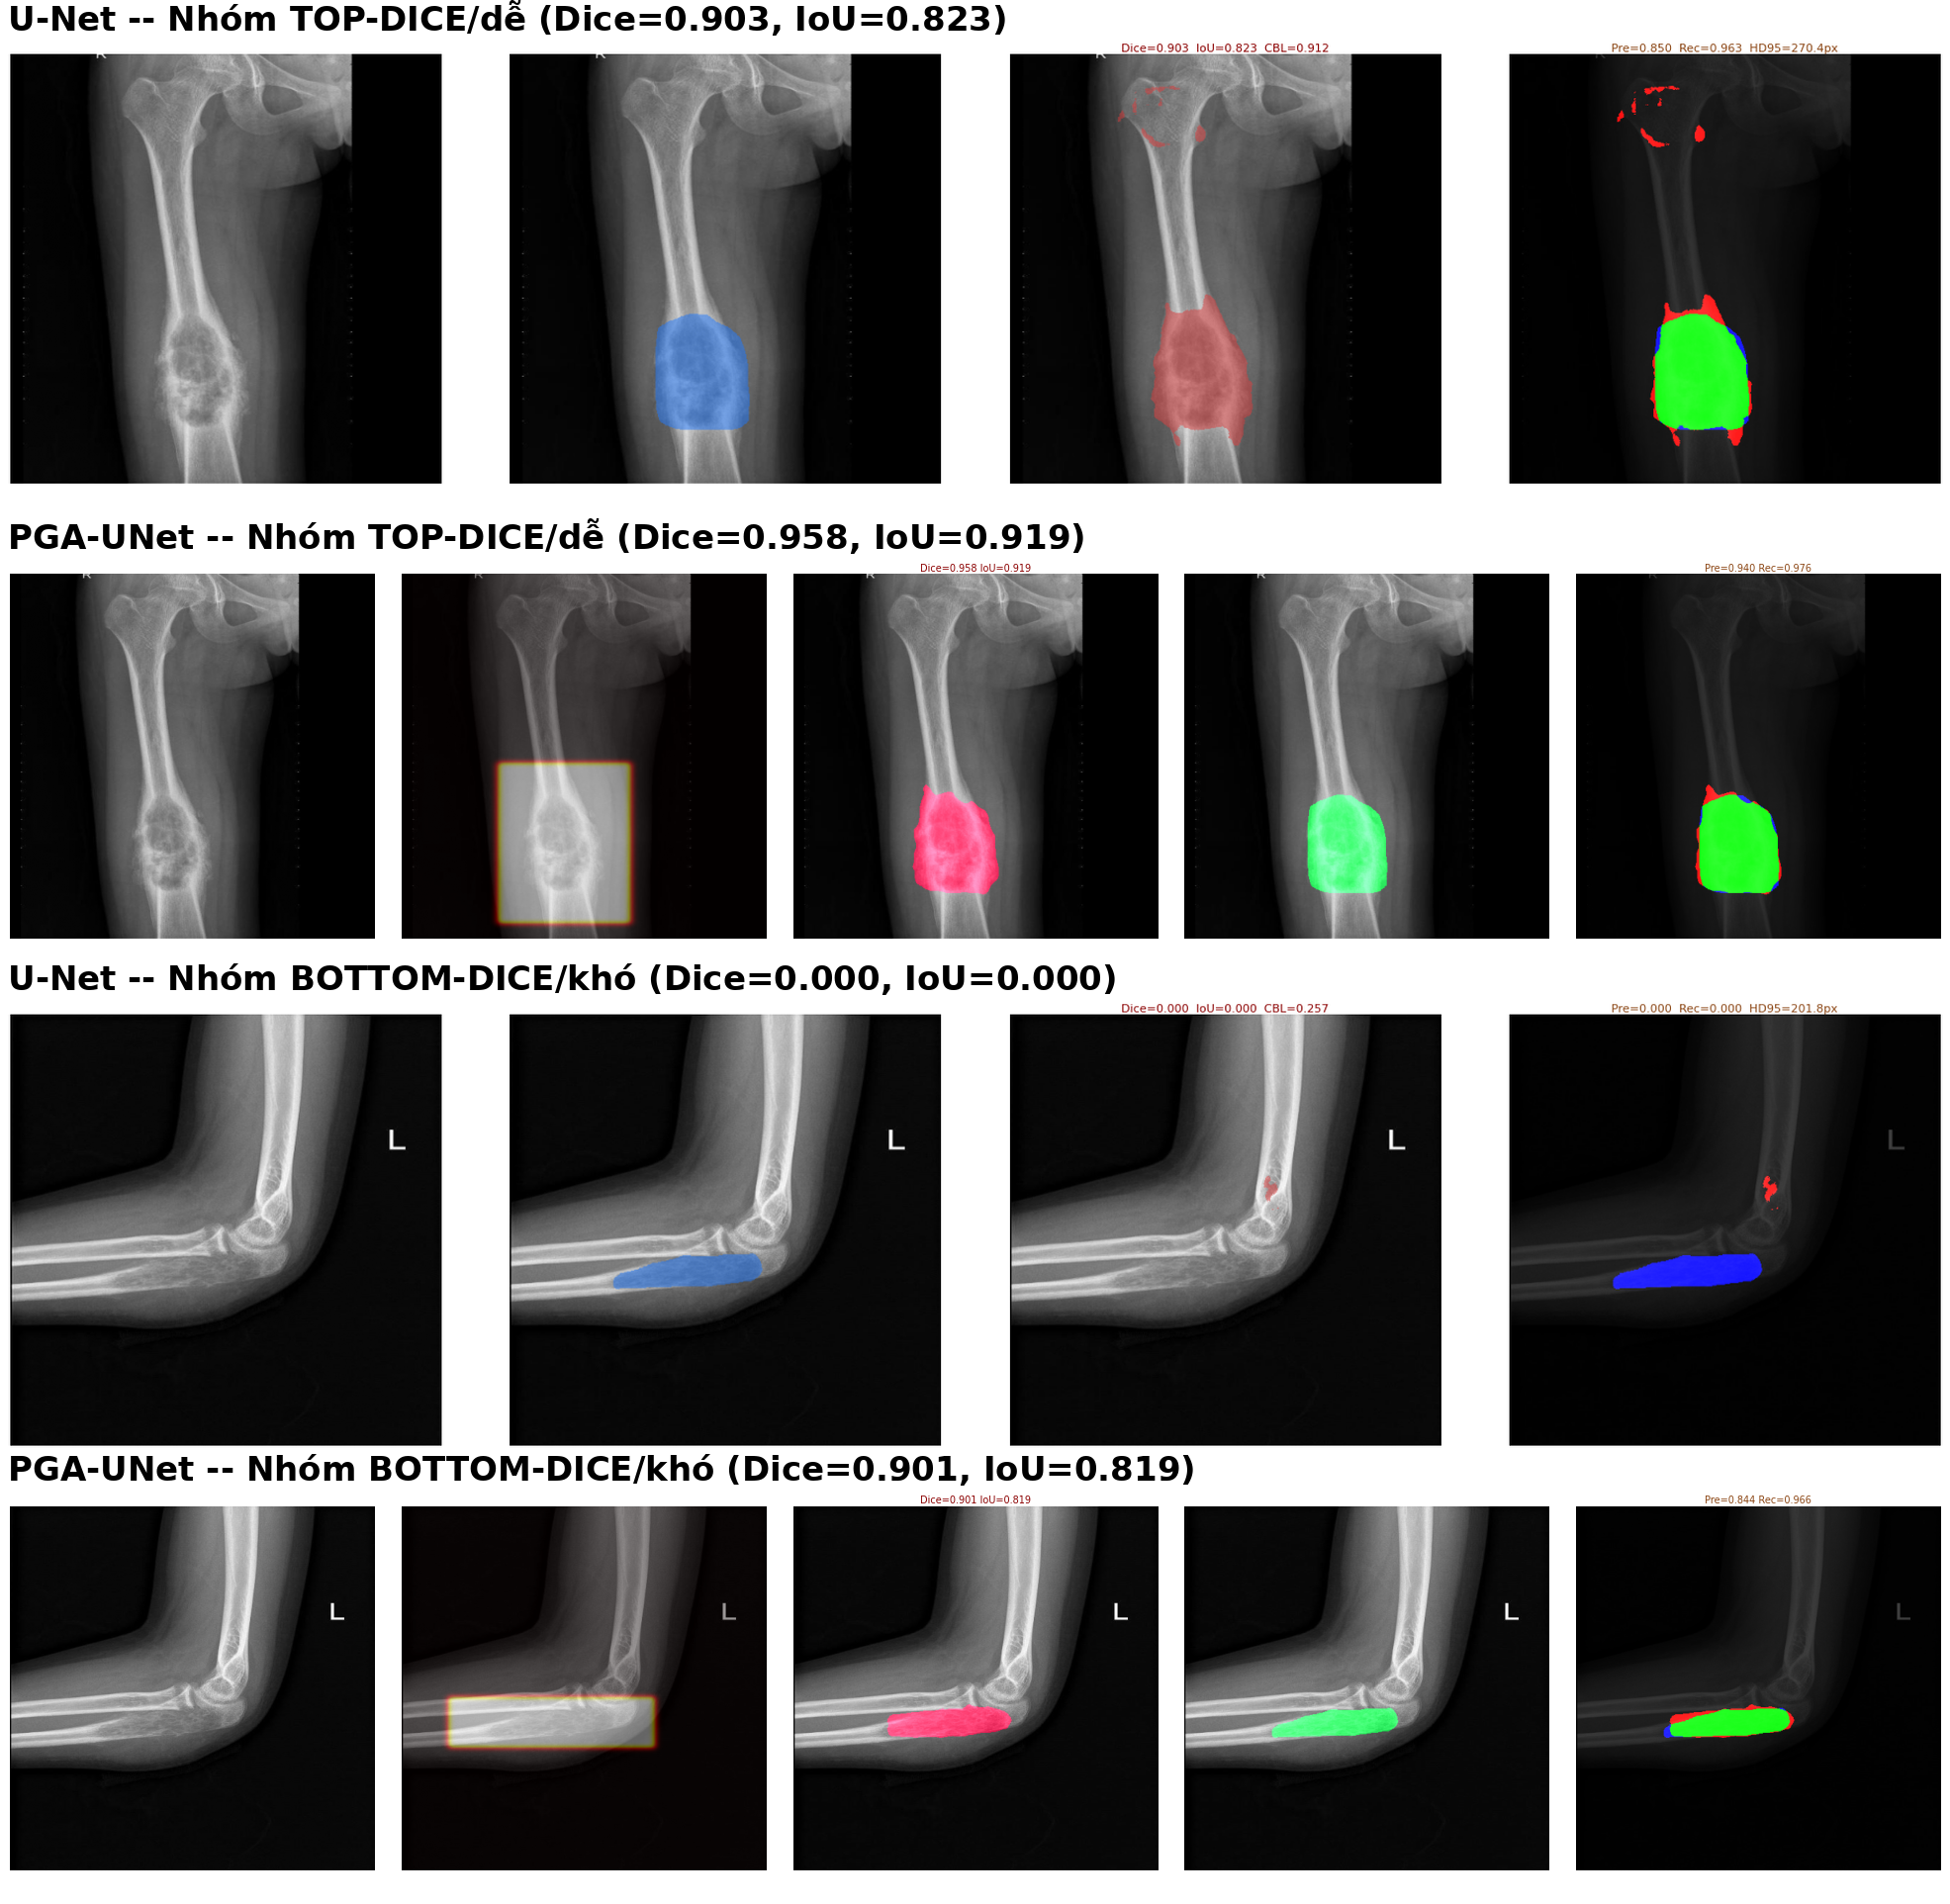
\includegraphics[width=\columnwidth]{images/unet_extreme_groups_btxrd.png}
\caption{Qualitative comparison between Attention U-Net and PGA-UNet on BTXRD for one case from the Attention U-Net top-Dice group and one case from the Attention U-Net bottom-Dice group.}
\label{fig:extreme-btxrd}
\end{figure}


\subsection{Matched Comparison with SAM-Med2D}
This comparison tests the architectural contribution of the proposed prompt handling against a prompt-based foundation baseline under matched input conditions. Both models receive the same prompt type and the same resolution, so the difference is more directly tied to how prompt information is represented and propagated. Table~\ref{tab:sam} therefore reports Dice at $256\times256$. PGA-UNet achieved higher Dice scores than fine-tuned SAM-Med2D under both evaluated prompt settings on both datasets. This matched comparison is more directly architectural because both models receive the same kind of coarse box prompt at the same resolution. The small-lesion analysis presented next should be read as an extension of this SAM-Med2D comparison to the setting where prompt usage is expected to matter most.

\begin{table}
\caption{Dice comparison with fine-tuned SAM-Med2D at $256\times256$.}
\label{tab:sam}
\centering
\resizebox{\columnwidth}{!}{%
\begin{tabular}{llcc}
\toprule
Dataset & Prompt & PGA-UNet & SAM-Med2D \\
\midrule
\multirow{2}{*}{BTXRD}
& Covering & \textbf{0.8433} & 0.7541 \\
& Off-center & \textbf{0.8150} & 0.6912 \\
\midrule
\multirow{2}{*}{FracAtlas}
& Covering & \textbf{0.8110} & 0.7339 \\
& Off-center & \textbf{0.7842} & 0.6743 \\
\bottomrule
\end{tabular}
}
\end{table}

Prompt robustness is one of the main observations. On BTXRD, Dice drops by 0.0283 when PGA-UNet moves from covering to off-center prompts, whereas SAM-Med2D drops by 0.0629. On FracAtlas, the corresponding drops are 0.0268 and 0.0596. In this setting, explicit prompt injection through PSG and CAD appears less sensitive to moderate prompt misalignment.


\subsection{Performance on Small Lesions}
This experiment is an extension of the SAM-Med2D comparison to the setting in which the contribution of prompt-aware feature preservation should be most visible, namely very small lesions. To keep subgroup analysis objective, we retain only the small-lesion subset because it is defined directly by lesion size rather than by a model-dependent ranking rule. For BTXRD, the subset is formed by selecting the 50 smallest lesions in the test set. This subset is then used for two related comparisons: PGA-UNet versus SAM-Med2D at the matched resolution of $256\times256$, and PGA-UNet$_{256}$ versus PGA-UNet$_{512}$ to examine the effect of resolution.

\begin{table}
\caption{Dice on the 50 smallest lesions in the BTXRD test set.}
\label{tab:small}
\centering
\resizebox{\columnwidth}{!}{%
\begin{tabular}{lcc}
\toprule
Model & Resolution & Dice \\
\midrule
SAM-Med2D & $256\times256$ & 0.1356 \\
PGA-UNet & $256\times256$ & 0.6870 \\
PGA-UNet & $512\times512$ & \textbf{0.8301} \\
\bottomrule
\end{tabular}
}
\end{table}

On this subset, PGA-UNet at $256\times256$ improves Dice by 0.5514 over SAM-Med2D at the same resolution. Increasing the PGA-UNet input size from $256\times256$ to $512\times512$ yields a further gain of 0.1431 Dice. These results are consistent with the view that small lesions benefit from both explicit prompt conditioning and higher spatial resolution.

One plausible explanation is that small lesions already provide limited visual evidence, and resizing a large radiograph to $256\times256$ weakens that evidence further. Under this condition, how prompt information is used becomes especially important. In SAM-Med2D, the box prompt primarily acts as a coarse positional cue for mask generation. When the lesion occupies very few pixels after resizing, this cue alone may be insufficient to recover a detailed mask. By contrast, PGA-UNet uses the bounding box as a dense spatial prior that amplifies the lesion region and propagates prompt information through both the encoder and decoder. This design appears better suited to preserving weak local evidence for small lesions. The stronger result of PGA-UNet at $512\times512$ is also consistent with this interpretation, since higher resolution preserves more lesion detail before prompt-guided decoding.

\begin{figure}[t]
\centering
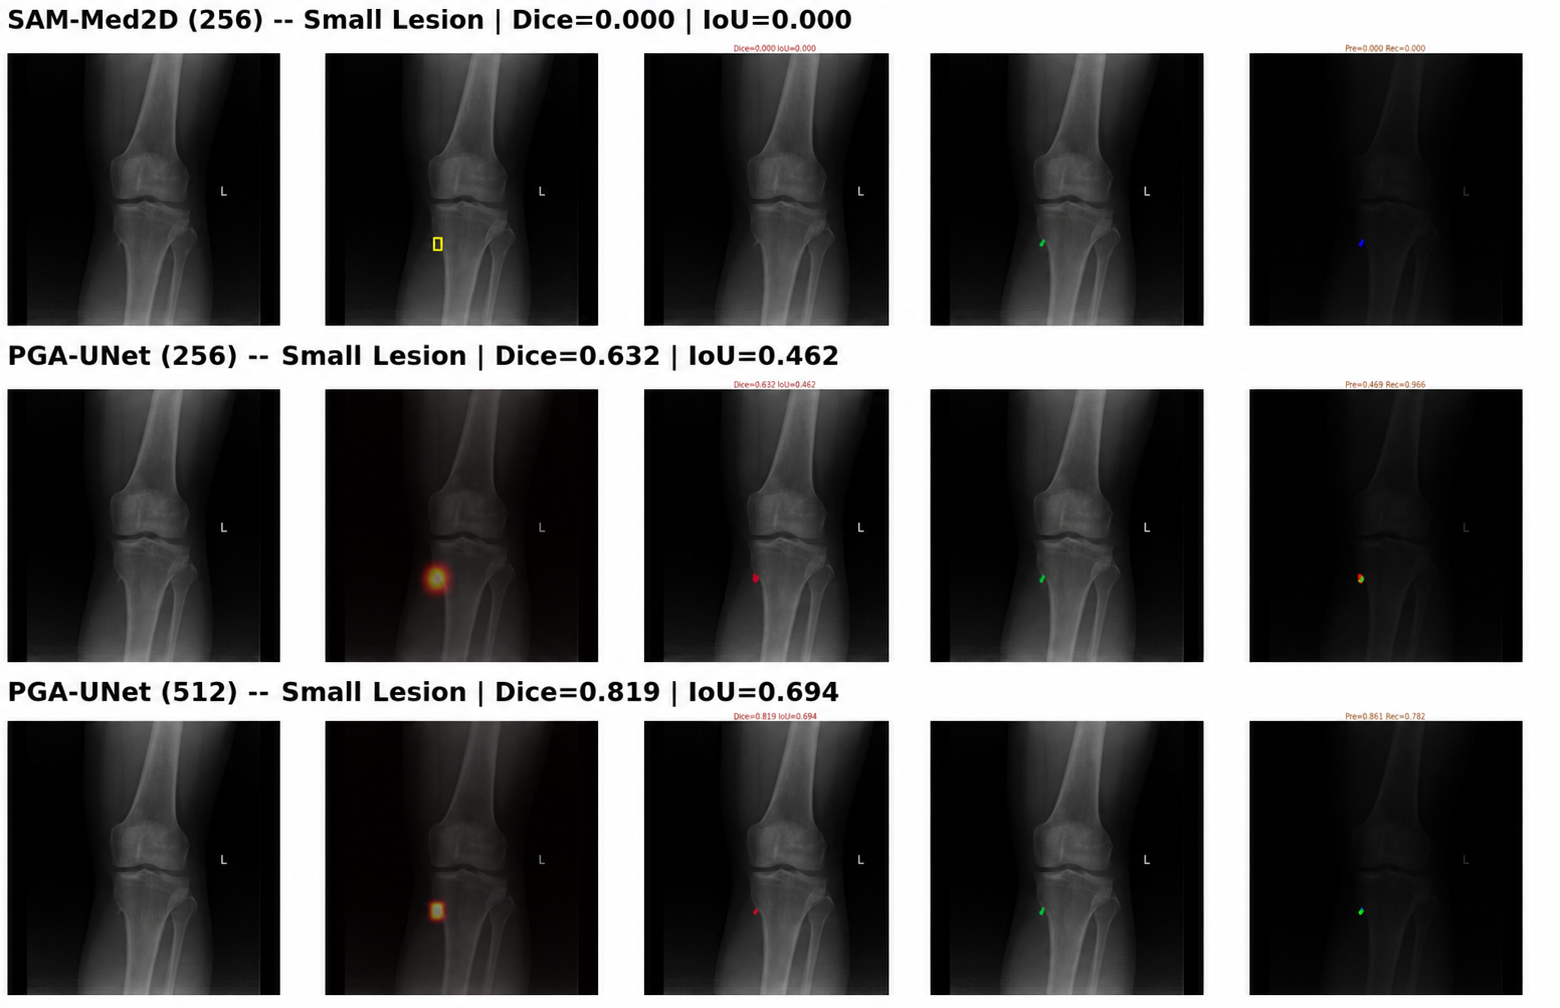
\includegraphics[width=\columnwidth]{images/small_lesion_sam_pga256_pga512.png}
\caption{Qualitative comparison on small lesions in BTXRD. The examples contrast SAM-Med2D at $256\times256$, PGA-UNet at $256\times256$, and PGA-UNet at $512\times512$.}
\label{fig:small-btxrd}
\end{figure}


\subsection{Efficiency Analysis}
This experiment evaluates whether the proposed gains are achieved with a practical computational profile. It supports the claim that the method is suitable for repeated low-latency interactive use rather than only for offline batch inference. Table~\ref{tab:efficiency} reports the efficiency comparison. PGA-UNet contains only 2.95M parameters. In the tested $256\times256$ setting, this corresponds to an approximately 92-fold reduction in parameter count and an 11.9-fold reduction in FLOPs relative to SAM-Med2D, together with 7.2$\times$ faster GPU inference.

\begin{table}
\caption{Efficiency comparison in the tested environment.}
\label{tab:efficiency}
\centering
\scriptsize
\resizebox{\columnwidth}{!}{%
\begin{tabular}{lccccc}
\toprule
Model & Params & GFLOPs & Size & GPU ms & CPU ms \\
\midrule
PGA-UNet 256 & 2.95M & 7.74 & 11.34 MB & 8.46 & 83.87 \\
PGA-UNet 512 & 2.95M & 30.97 & 11.34 MB & 21.83 & 309.84 \\
SAM-Med2D 256 & 271.24M & 92.02 & 2443.16 MB & 60.70 & 769.40 \\
\bottomrule
\end{tabular}
}
\end{table}


\subsection{Ablation Study}
The ablation study directly tests which proposed components are responsible for the observed gains. In particular, it examines whether performance comes from the prompt itself, from encoder-side prompt gating, from decoder-side prompt-conditioned attention, or from the combination of all three. The clearest ablation gains appear under off-center prompts rather than under ideal prompts. Table~\ref{tab:ablation} summarizes the main configurations retained in the article. The ablation set isolates the roles of Gaussian prompting, PSG, CAD, and the original Attention U-Net gate. Relative to the concatenated-prompt baseline, the full PGA-UNet trades a small amount of Dice under ideal covering prompts for markedly better robustness under off-center prompts on both datasets.

\begin{table}
\caption{Summary ablation results (Dice) for the main prompt-aware configurations at $512\times512$.}
\label{tab:ablation}
\centering
\scriptsize
\resizebox{\columnwidth}{!}{%
\begin{tabular}{llcc}
\toprule
Dataset & Configuration & Covering & Off-center \\
\midrule
\multirow{3}{*}{BTXRD}
& Concatenated prompt baseline & 0.8763 & 0.7364 \\
& Best covering configuration & \textbf{0.8861} & 0.7406 \\
& PGA-UNet & 0.8607 & \textbf{0.8423} \\
\midrule
\multirow{3}{*}{FracAtlas}
& Concatenated prompt baseline & 0.8131 & 0.6579 \\
& Best covering configuration & \textbf{0.8351} & 0.6927 \\
& PGA-UNet & 0.8169 & \textbf{0.7850} \\
\bottomrule
\end{tabular}
}
\end{table}

Replacing the original Attention U-Net gate with CAD improves off-center Dice by 0.1065 on BTXRD and 0.0924 on FracAtlas. Replacing a binary prompt with the Gaussian plateau prompt improves off-center Dice by 0.0990 and 0.1005, respectively. These are the largest and most consistent gains observed in the component study.

An important nuance is that the best configuration depends on the prompt condition. In the covering setting, a reduced variant with prompt-aware decoding can still achieve the highest score among the ablation configurations on BTXRD. However, the full proposed PGA-UNet is the strongest configuration under off-center prompts, where robustness to prompt misalignment is the primary goal of the design. This trade-off is consistent with the intended use case, since practical interaction is more likely to include mildly imperfect box placement than perfectly aligned prompts. Taken together, the ablation results indicate that the Gaussian prompt, PSG, and CAD each contribute useful behavior individually, but the full combination of all three components provides the strongest overall prompt-robust configuration.

\begin{figure}[t]
\centering
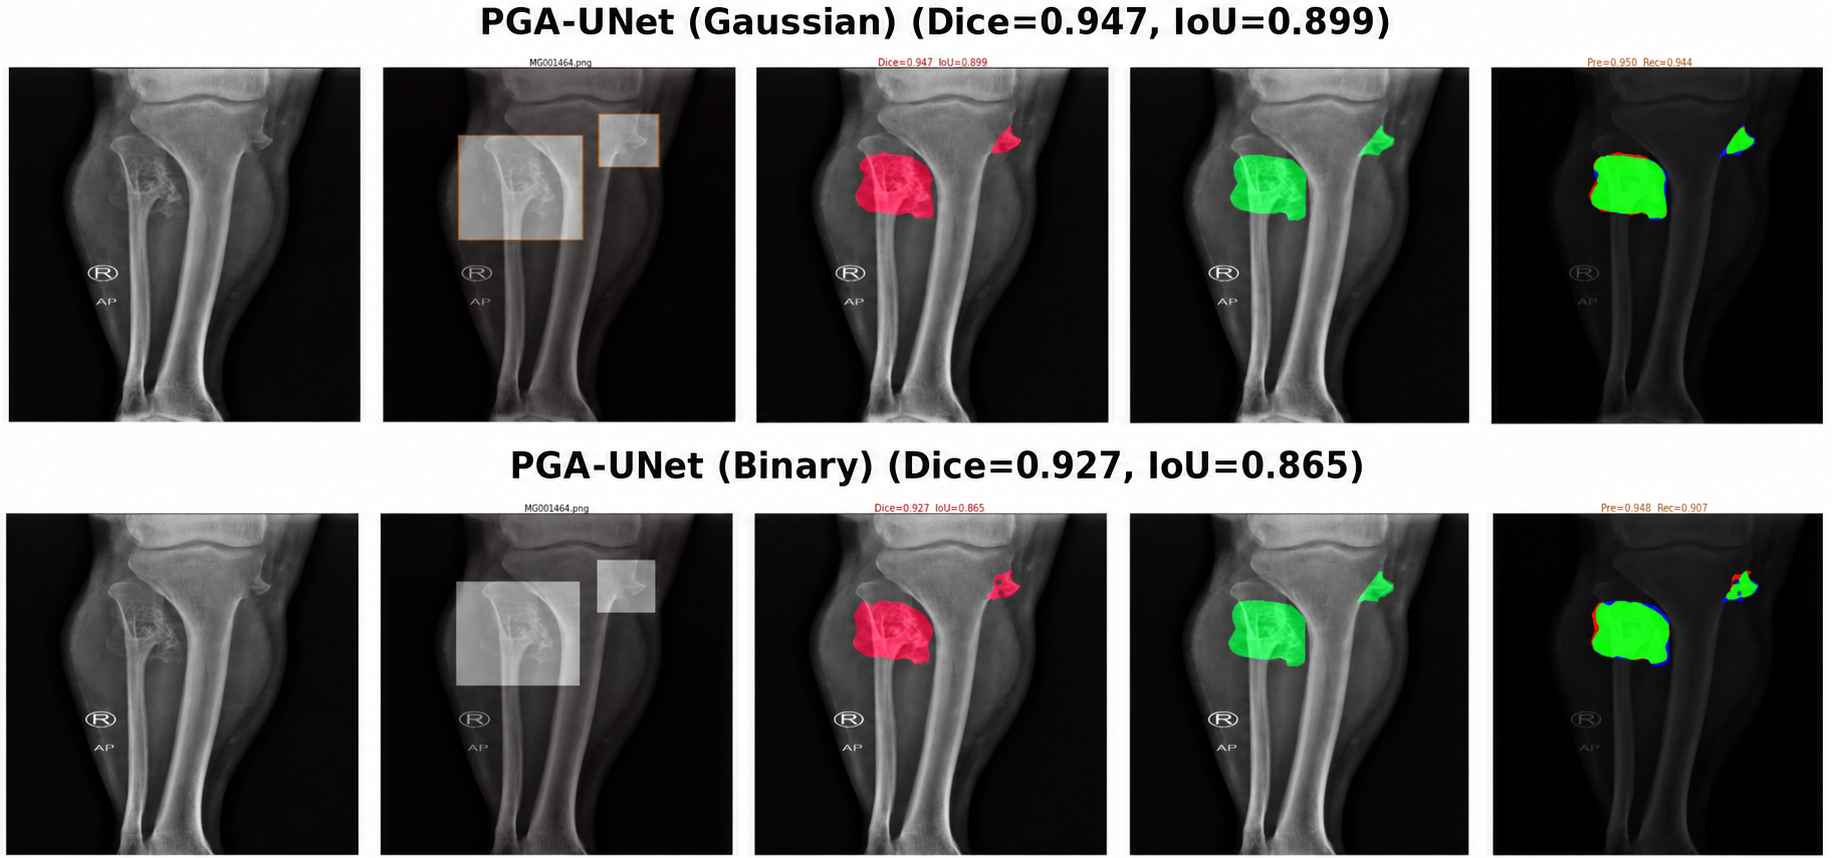
\includegraphics[width=\columnwidth]{images/ablation_gaussian_vs_binary_case.png}
\caption{Qualitative comparison between the Gaussian prompt representation and the binary prompt representation. The Gaussian version produces cleaner boundaries and better overlap on this representative BTXRD example.}
\label{fig:ablation-gaussian-binary}
\end{figure}

\subsection{Failure Modes}
The method still has identifiable failure cases. In the qualitative review collected during the thesis experiments, lower Dice scores were more likely for lesions with highly elongated or branching shapes, lesions located in anatomically cluttered regions such as the shoulder or clavicle, and lesions with weak contrast relative to surrounding structures. These cases are relevant because they show that prompt guidance does not eliminate ambiguity once the local image evidence itself is poor.

\begin{figure}[t]
\centering
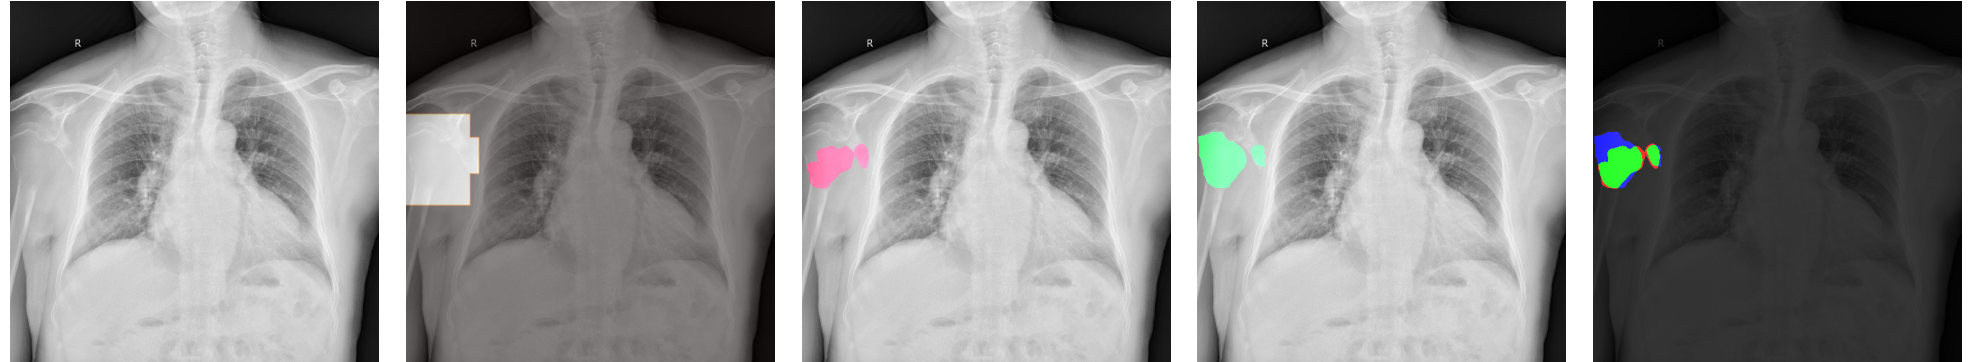
\includegraphics[width=\columnwidth]{images/failure_case_overlap.png}
\caption{Representative failure case in an anatomically overlapping region. Even with a covering prompt, the lesion boundary remains difficult because the local X-ray structures are visually confounded.}
\label{fig:failure}
\end{figure}

\section{Discussion}
The results support several main observations. First, PGA-UNet performs well on both datasets. Second, compared with the stronger automatic baseline Attention U-Net, PGA-UNet achieves higher system-level segmentation performance when coarse box guidance is available. Third, compared with SAM-Med2D at the matched prompt setting and matched $256\times256$ resolution, PGA-UNet again performs better. Fourth, the advantage becomes even clearer on the small-lesion subset. Fifth, the ablation results confirm that the Gaussian prompt, PSG, and CAD each contribute to the final behavior. Finally, the efficiency analysis shows that the model remains substantially lighter and faster than SAM-Med2D.

The scope of the analysis was deliberately narrowed. The auxiliary screening pipeline is excluded because it addresses a different question from prompt-guided segmentation itself. Likewise, the retained subgroup analyses are objective constructions tied either to lesion size or to a baseline-defined ranking.

The current study still has limitations. The model depends on resizing inputs to a fixed resolution, which can dilute fine lesion detail in very small targets. The current formulation does not yet exploit additional information sources beyond the image and box prompt, and the training setup still requires dense mask supervision. The evaluation also remains limited to the current public datasets. Prompts are simulated from annotations rather than collected from radiologists, and BTXRD and FracAtlas are evaluated in separate retraining settings rather than through external-domain transfer. Finally, the main robustness claims are supported by the current deterministic split and ablation results, not by repeated multi-seed reporting.

An additional limitation is interpretive rather than purely empirical. Several observed gains, especially under prompt perturbation, are consistent with the intended roles of PSG, CAD, and the Gaussian plateau prompt, but this article does not include feature-level probing that would establish a unique internal mechanism for those gains. The ablation study therefore supports the usefulness of the design choices at the system level, not a definitive causal account of representation dynamics inside the network.

\section{Conclusion}
This article presented PGA-UNet, a lightweight prompt-guided CNN for interactive bone X-ray lesion segmentation. By combining a plateau-style Gaussian prompt map with encoder-side Prompt Spatial Gates and decoder-side Conditional Attention Decoders, the model achieves favorable results on BTXRD and FracAtlas while remaining substantially smaller than SAM-Med2D. The most consistent evidence for the design lies in robustness under imperfect prompts, strong performance on the 50 smallest BTXRD lesions relative to SAM-Med2D, and greater stability on Attention U-Net-defined failure cases. Future work should evaluate the method with radiologist-provided prompts, external cohorts, higher-resolution processing without aggressive resizing, and broader clinical interaction settings.

\section*{Data Availability}
BTXRD and FracAtlas are public datasets cited in this article. The manuscript reports experiments on image-level train/validation/test splits derived from those datasets. Code and split details should be released with the final reproducibility package.

\section*{Author Contributions}
Thong Luc: conceptualization, methodology, software, investigation, formal analysis, visualization, writing of the original draft. Nguyen Huu Binh: software support, data preparation, experiment verification, review and editing. Ly Quoc Ngoc: supervision, validation, review and editing.

\section*{Ethics Statement}
This study used public de-identified radiograph datasets and did not involve prospective data collection, patient contact, or intervention.

\section*{Acknowledgment}
OpenAI ChatGPT was used only for vocabulary and grammar refinement in selected non-technical manuscript text. All technical content, experimental design, mathematical formulation, figures, tables, and conclusions were prepared and verified by the authors, who take full responsibility for the final manuscript.

\begin{thebibliography}{00}
\bibitem{b1} A. Kirillov \textit{et al.}, ``Segment Anything,'' in \textit{Proc. IEEE/CVF Int. Conf. Comput. Vis.}, 2023, pp. 4015--4026.
\bibitem{b2} J. Cheng \textit{et al.}, ``SAM-Med2D,'' \textit{arXiv preprint arXiv:2308.16184}, 2023.
\bibitem{b3} O. Ronneberger, P. Fischer, and T. Brox, ``U-Net: Convolutional Networks for Biomedical Image Segmentation,'' in \textit{MICCAI}, 2015, pp. 234--241.
\bibitem{b4} O. Oktay \textit{et al.}, ``Attention U-Net: Learning Where to Look for the Pancreas,'' in \textit{Medical Imaging with Deep Learning}, 2018.
\bibitem{b5} N. Xu, B. Price, S. Cohen, J. Yang, and T. S. Huang, ``Deep Interactive Object Selection,'' in \textit{Proc. IEEE Conf. Comput. Vis. Pattern Recognit.}, 2016, pp. 373--381.
\bibitem{b6} G. Wang \textit{et al.}, ``DeepIGeoS: A Deep Interactive Geodesic Framework for Medical Image Segmentation,'' \textit{IEEE Trans. Pattern Anal. Mach. Intell.}, vol. 41, no. 7, pp. 1559--1572, 2019.
\bibitem{b7} S. Yao \textit{et al.}, ``A Radiograph Dataset for the Classification, Localization, and Segmentation of Primary Bone Tumors,'' \textit{Scientific Data}, vol. 12, no. 1, p. 88, 2025.
\bibitem{b8} I. Abedeen \textit{et al.}, ``FracAtlas: A Dataset for Fracture Classification, Localization and Segmentation of Musculoskeletal Radiographs,'' \textit{Scientific Data}, vol. 10, no. 1, p. 521, 2023.
\bibitem{b9} J. Ma \textit{et al.}, ``Segment Anything in Medical Images,'' \textit{Nat. Commun.}, vol. 15, no. 1, p. 654, 2024.
\end{thebibliography}

\begin{IEEEbiography}[{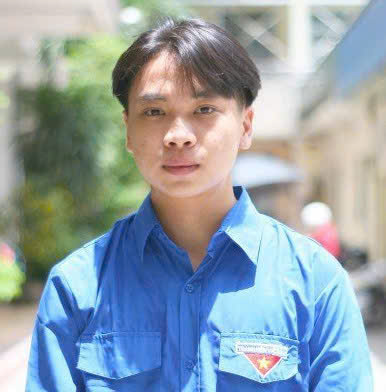
\includegraphics[width=1in,height=1.25in,clip,keepaspectratio]{images/author_thong_luc.jpg}}]{Thong Luc}
Thong Luc is a final-year undergraduate student in the B.Sc. program in Computer Science with the Faculty of Information Technology, University of Science, Vietnam National University Ho Chi Minh City, Vietnam. His research interests include computer vision, deep learning, medical image analysis, image segmentation, and interactive prompt-guided segmentation. His current work focuses on prompt-guided segmentation for bone radiographic images using deep learning.
\end{IEEEbiography}

\begin{biographynophoto}{Nguyen Huu Binh}
Nguyen Huu Binh is currently an undergraduate student in Computer Science with the Faculty of Information Technology, University of Science, Vietnam National University Ho Chi Minh City, Vietnam. His research interests include computer vision, deep learning, and image segmentation. His current research focuses on deep learning methods for medical image segmentation using visual prompts.
\end{biographynophoto}

\begin{biographynophoto}{Ly Quoc Ngoc}
[ Th\`ay \dj i\`en th\^ong tin gi\'up em: biography ]
\end{biographynophoto}

\EOD
\end{document}
